%!TEX root = ../main.tex

\section{Halleffekt}

\section{Galiumarsenid}
Bei der zweiten Probe handelt es sich um eine modulationsdotierte GaAs/AlGaAs Heterostruktur, diese bildet ein 2-dimensionales Elektronengas aus. 
\subsection{Beweglichkeit}
Analog zur Germanium Probe im unipolaren (extrinsischen) Fall wird die die Beweglichkeit berechnet via:
\begin{equation}
    \mu = \sigma |R_H|.
\end{equation}
Aufgrund der Van-der-Pauw-Geomatrie ("Kreuz-Form") berechnet sich die Leitfähigkeit und der Hallkoeffizient im 2-dimensionalen Fall (2DEG) mit:
\begin{align}
    \sigma &= \frac{ln(2)}{\pi} \frac{I}{U_L} \\
    R_H &= \frac{\Delta U_H}{I} \frac{1}{B}.
\end{align}
In Abbildung $\autoref{fig:GaAs_Bew}$ erkennt man eine abnehmende Beweglichkeit mit hohen Temperaturen. Dies ist vor allem der zunehmenden Streuung polar-optischen Phononen und akustischen Phononen geschuldet.  
\begin{figure}
    \centering
    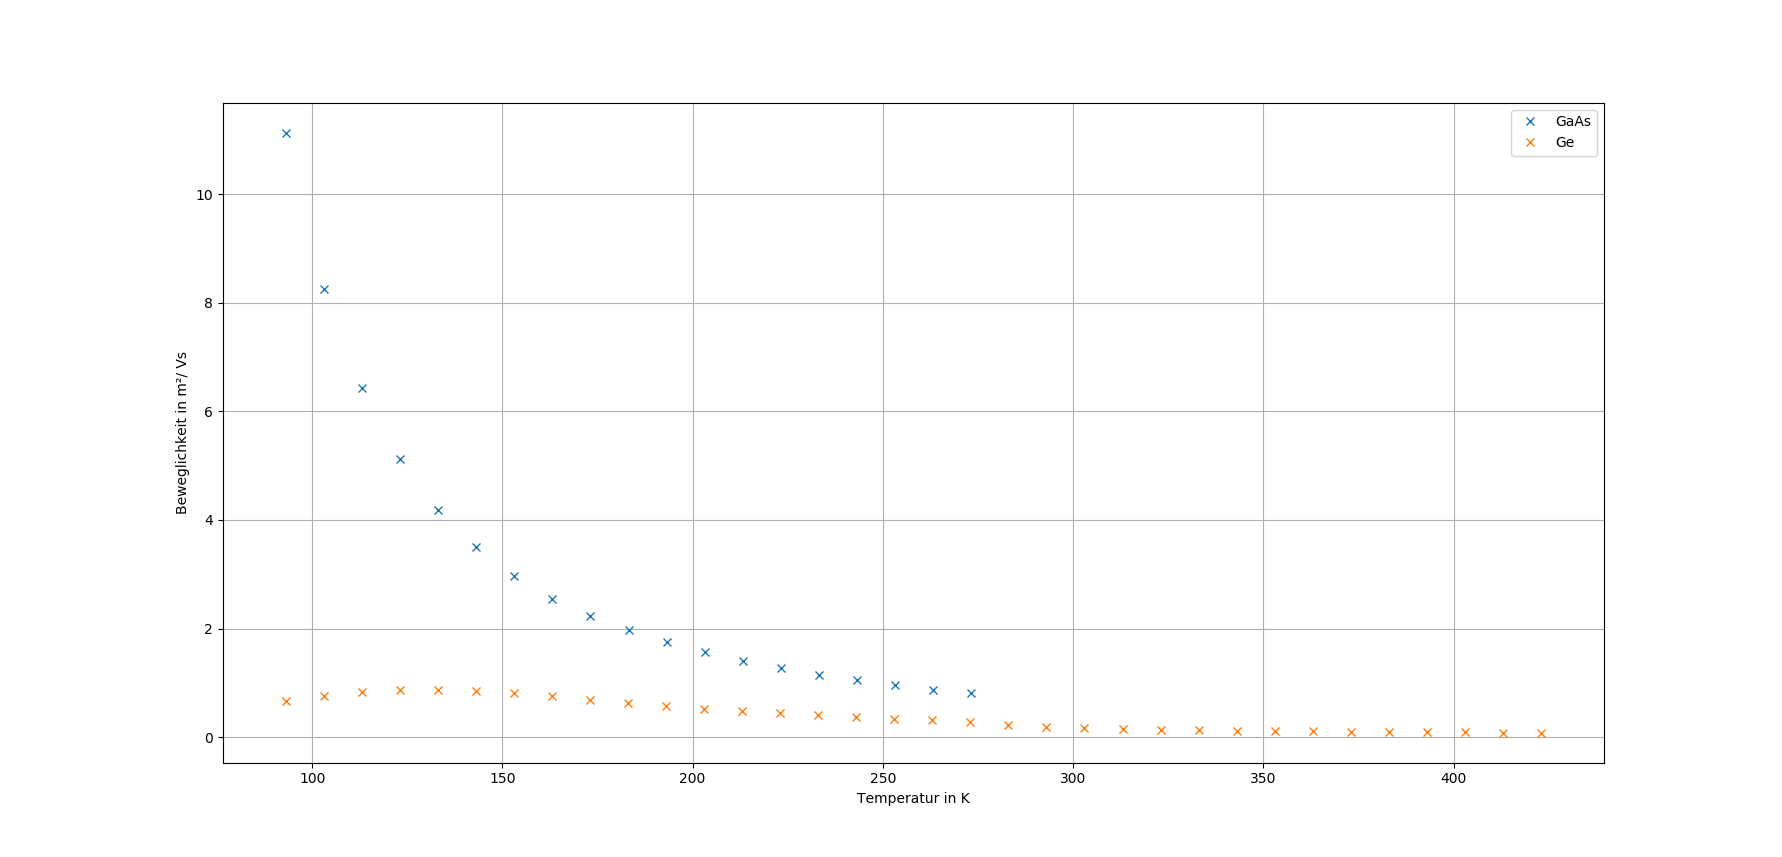
\includegraphics[width=1.0\textwidth]{./fig/GaAs_bew.png}
    \caption{Beweglichkeit von Ge und GaAs im Vergleich}
    \label{fig:GaAs_Bew}
\end{figure}

Vergleicht man die Beweglichkeiten von Germanium und GaAs erkennt man ein deutlichen Unterschied der Beweglichkeit vor allem bei niedrigen Temperaturen. Dies liegt daran, dass für Germanium die Streuung an geladener Störstellen dominiert. Bei niedrigen Temperaturen nimmt die Geschwindigkeit der Teilchen ab und die Ablenkung durch das Coulomb-Potential zu, daher sinkt die Stoßzeit und somit die Beweglichekeit. 
Es ist abzusehen, dass für noch tiefere Temperaturen die Beweglichkeit von GaAs zunimmt.

\begin{table}[]
    \centering
    \begin{tabular}{c|c}
    \hline
         Temperatur in K & Beweglichkeit in $\frac{m^2}{Vs}$\\
         \hline
         93,15& 11,13$\pm$ 0,26\\
         103,15&8,26 $\pm$ 0,19   \\
         113,15&6,42   $ \pm$ 0,15    \\
         123,15&5,15   $\pm $0,15     \\
         133,15&4,17    $\pm $ 0,09   \\
         143,15&3,51$\pm $0,08        \\
         153,15&2,96  $ \pm$ 0,07     \\
         163,15&2,55    $ \pm$ 0,06   \\
         173,15&2,23     $\pm$ 0,05   \\
         183,15&1,97   $\pm $0,05     \\
         193,15&1,76  $\pm $0,04      \\
         203,15&1,56   $\pm $0,04     \\
         213,15&1,41   $\pm$0,04     \\
         223,15&1,27   $\pm $0,04     \\
         233,15&1,15    $ \pm$0,03   \\
         243,15&1,05   $\pm $0,03     \\
         253,15&0,95    $ \pm$0,03   \\
         263,15&0,88    $\pm $0,03    \\
         273,15&0,80    $\pm $0,03    \\
         \hline
    \end{tabular}
    \caption{Beweglichkeit von GaAs bei verschiedenen Temperaturen}
    \label{tab:GaAs_web}
\end{table}